% !TEX program = xelatex
% Пример: статья «Исследование возможности детектирования светофоров»
% Источник: Article_1.docx
\documentclass{misisarticle}

\grnti{47.01.07, 47.01.09}
\asjc{1707, 2207}
\oecd{1020, 1070}

\title{Исследование возможности детектирования светофоров}

\misisauthor{Л.~С.~Толстенко}{кафедра инженерной кибернетики НИТУ «МИСиС»}{Москва, Россия}{m1805775@edu.misis.ru}
\misisauthor{А.~А.~Клейменов}{кафедра инженерной кибернетики НИТУ «МИСиС»}{Москва, Россия}{m1801083@edu.misis.ru}
\misisauthor{Р.~Н.~Садеков}{кафедра инженерной кибернетики НИТУ «МИСиС»}{Москва, Россия}{r.sadekov@misis.ru}

\setabstract{в настоящее время широкое распространение получают беспилотные системы управления различными транспортными средствами, в том числе автомобилями. Управление беспилотным автомобилем предполагает решение задач, связанных с распознаванием объектов дорожной обстановки: пешеходов, автомобилей, препятствий (в виде ям и т. д.), дорожных знаков, разметки, светофоров. Автономные наземные транспортные средства должны быть способны воспринимать сигналы светофора, чтобы ездить по улицам вместе с водителями-людьми. В большинстве случаев водитель-человек может легко идентифицировать соответствующие сигналы светофоров. Методы глубокого обучения показали высокую производительность и точность в данной области. В работе рассматриваются несколько решений с открытым исходным кодом и сравниваются возможности распознавания светофоров по изображениям со стереокамеры на наборе данных LISA.}
\setkeywords{Компьютерное зрение, Детекция светофоров, Распознавание светофоров, Монокулярная камера, Беспилотные автомобили, YOLO, mAP, LISA}

\begin{document}
\maketitle

\section{Введение}

Изучением и проектированием беспилотных автомобилей занимаются многие университеты, научно-исследовательские центры, автомобильные и иные промышленные компании по всему миру с середины 1980-х годов. Известны разработки беспилотных транспортных средств, созданные гигантами автомобилестроения (Ford, Honda, Mercedes, Tesla, КАМАЗ совместно с Cognitive Technologies), ИТ-компаниями (Uber, Google, Яндекс) [1].

При создании системы управления беспилотного автомобиля важными задачами являются обнаружение и распознавание объектов дорожной обстановки. Для решения применяются технологии компьютерного зрения. В числе задач по обнаружению/распознаванию объектов в видеопотоке с камеры, установленной на автомобиль, можно выделить задачу идентификации световых сигналов, подаваемых светофорами.

Обнаружение и распознавание сигнала светофора включает в себя непосредственно его обнаружение и распознавание состояния (красный, зелёный или жёлтый). В литературе описаны различные способы решения этой задачи [2], в том числе и при наличии неблагоприятных погодных условиях (слабая освещённость, дымка, туман и т. д.) [3].

Методы глубокого обучения показали высокую производительность и способность к обобщению во многих областях и типах задач, таких как классификация [4, 5] и обнаружение [6]. Детекторы объектов общего назначения были хорошо изучены для задач, связанных с дорожным движением (таких как обнаружение светофоров, дорожных знаков и т. д.). YOLO [7] и R-CNN [8] являются двумя из этих современных детекторов. В работе рассматриваются и сравниваются достижения (с открытым исходным кодом) в области глубокого обучения для определения местоположения (и дальнейшего распознавания) светофоров по изображениям 2D-камеры.

Подходы, основанные на обучении, особенно те, которые используют глубокое обучение, требуют больших объёмов аннотированных данных, что не всегда есть в наличии. В настоящее время в свободном доступе есть зарубежные базы изображений с аннотациями светофоров [9, 10, 11]. Однако следует также заметить, что подходы, основанные на обучении, требуют больших вычислительных мощностей.

\section{Наборы данных}

Для обучения и тестирования рассматриваемых в данной работе нейросетей использовались некоторые наборы данных, как локальные, собранные авторами, так и открытые. Рассмотрим используемые открытые наборы.

\subsection{LISA}

Обширный набор общедоступных данных LISA [9], основанный на кадрах с дорог Сан-Диего штата Калифорния, содержит аннотированные видеопоследовательности, снятые при разном освещении (различное время суток) и погодных условиях с помощью стереокамеры (рисунок 1). Кроме того, в наборе данных представлены многосекционные светофоры, которые помимо цвета имеют и направления – всего 7 классов (рисунок 2): go, goForward, goLeft, stop, stopLeft, warning, warningLeft.

На рисунке 3 отображены некоторые нетривиальные случаи возникновения светофоров в кадре:

\begin{itemize}
  \item смещение цветового тона и нарушение ореола из-за атмосферных условий и влияния других источников света (а, б, в, г);
  \item полное или частичное перекрытие другими объектами или непрямой угол обзора (д, е, ж, з);
  \item неполная форма светофора из-за неисправной или грязной лампы (и);
  \item стоп-сигналы автомобилей, отражения, рекламные щиты и огни пешеходных переходов (к);
  \item проблемы синхронизации между скоростью затвора камеры и рабочим циклом светофора (л, м).
\end{itemize}
\begin{figure}[htbp]
  \centering
  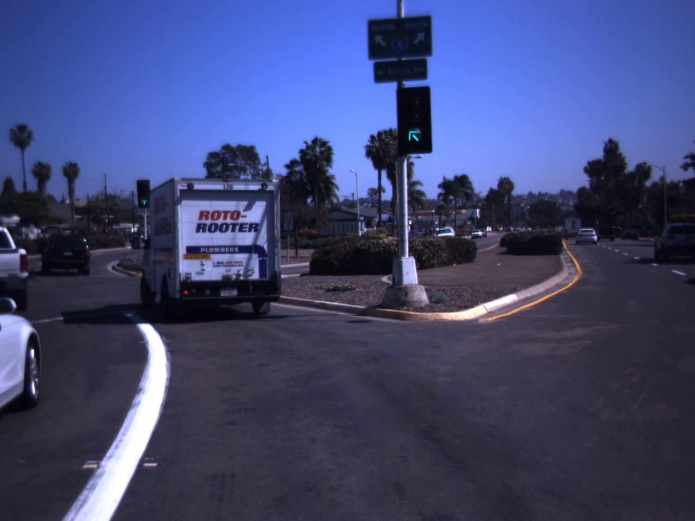
\includegraphics[width=\columnwidth]{figures/example/fig01.jpeg}
  \caption{Примеры кадров при дневном и ночном освещении}
  \label{fig:1}
\end{figure}

\begin{figure}[htbp]
  \centering
  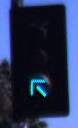
\includegraphics[width=\columnwidth]{figures/example/fig02.png}
  \caption{Примеры классов состояния светофора: а) go, б) goForward, в) goLeft, г) stop, д) stopLeft, е) warning, ж) warningLeft}
  \label{fig:2}
\end{figure}

\subsection{DriveU}

Набор данных DriveU [12] содержит около 230000 ручных аннотаций кадров, снятых в 11 разных городах при разных погодных условиях. Разметка кадров содержит в себе информацию об:

ограничивающих светофоры прямоугольниках;

состоянии (цвет светофора);

релевантности (относится ли светофор к текущему движению);

горизонтальной или вертикальной ориентации;

наличии визуального перекрытия;

количестве светодиодов, типе светофора (для пешеходов, велосипедистов или автомобилей).

Запись видеопоследовательностей велась при помощи стерео и широкоугольной камер. По стереопаре изображений также строится карта несоответствия [13] (рисунок 4).

\begin{figure}[htbp]
  \centering
  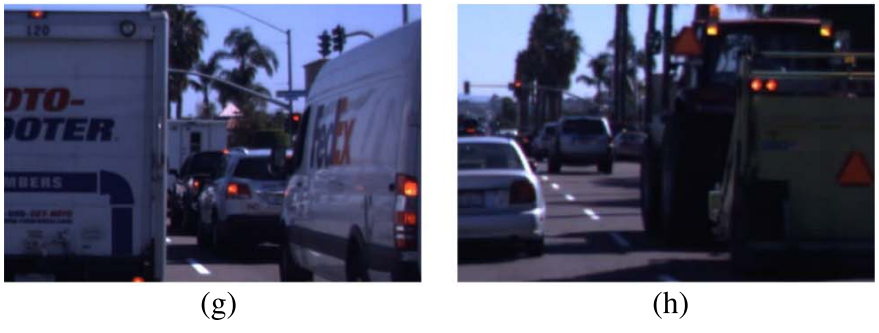
\includegraphics[width=\columnwidth]{figures/example/fig03.png}
  \caption{Примеры сложных ситуаций возникновения светофоров в кадре}
  \label{fig:3}
\end{figure}

\begin{figure}[htbp]
  \centering
  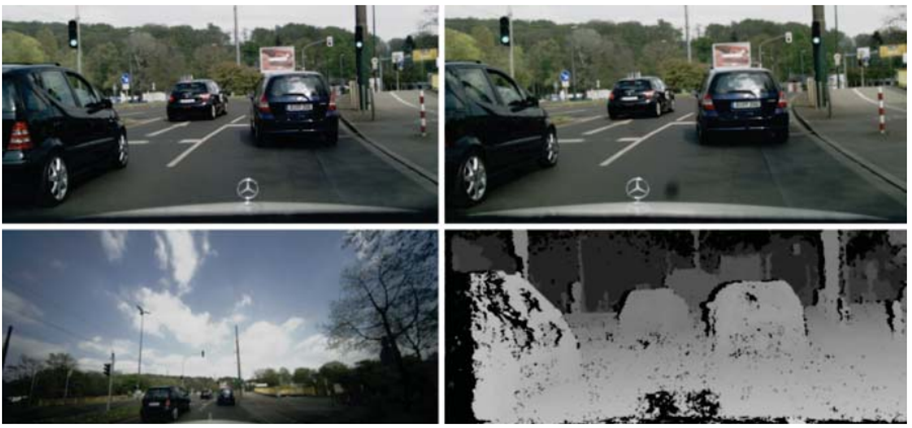
\includegraphics[width=\columnwidth]{figures/example/fig04.png}
  \caption{Пример кадра видеопоследовательности: два верхних изображения образуют стереопару, левое нижнее – соответствующий кадр широкоугольной камеры, правое нижнее – карта несоответствия}
  \label{fig:4}
\end{figure}

\section{Нейросетевые архитектуры}

\subsection{Модификация YOLOv3 на фреймворке Darknet}

В работе [14] решается задача распознавания релевантных светофоров для применения в беспилотных автомобилях. Авторы предлагают использовать детектирующую нейронную сеть, локализующую и распознающую светофоры в кадре, в сочетании с prior map – разметкой предопределённых маршрутов, в которой содержится информация о позиции, направлении и других характеристиках реальных светофоров, благодаря чему беспилотный автомобиль будет заранее иметь информацию о наличии светофора в кадре. Благодаря такому подходу авторам статьи удаётся определить, стоит ли брать во внимание состояние того или иного светофора в зависимости от того, относится ли он к текущему движению или попал в кадр случайно.

Разработка конечной системы велась в две стадии:

\begin{itemize}
  \item в течение оффлайн-фазы были построены prior карты с использованием лидара и размечены релевантные светофоры;
  \item онлайн-фаза заключается в распознавании светофоров на кадрах видеопоследовательностей, выделении (при помощи разметки оффлайн-фазы) релевантных светофоров среди найденных (рисунок 6), и определении их состояния – «none», «off», «red», «green».
  \item Для текущей работы представляет интерес нейросетевая часть онлайн-фазы – детектирование и распознавание светофоров в кадре. Авторы [14] используют YOLOv3 [15], в основе которой лежит Darknet-53 (рисунок 7). Данная модель была обучена для детектирования и распознавания состояния светофора. Нейронная сеть на выходе имеет два класса – «red», в котором объединены красный и жёлтый цвет, и «green». Авторами отмечается, что красный и жёлтый цвет пришлось объединить в один класс из-за недостаточного количества данных с жёлтым цветом светофора, и как следствие невозможностью обучить нейронную сеть достаточного качества для данного класса.
  \item Открытые наборы данных DriveU и LISA были использованы для обучения и тестирования нейронной сети. Кроме того, был собран локальный датасет, названный авторами IARA, содержащий около 5000 размеченных светофоров и 3-классовую разметку («red», «green», «yellow»), на котором дополнительно проводилось тестирование. В качестве функции потерь использовалась mAP [16] – mean Average Precision для каждого класса, который в свою очередь, считается как площадь под кривой precision-recall.
  \item (1)
\end{itemize}
YOLOv3 обучалась на 1500 батчах по 64 изображения в каждом и с константным learning rate = . Размер изображений составляет 608х608 пикселей – компромисс между скоростью и качеством.

Также в процесс обучения были включены: аугментация изображений при помощи изменения оттенка, насыщенности, экспозиции, батч-нормализация. Кроме того, каждые 10 батчей менялось разрешение изображений с 608х608 на разрешения, кратные 32, что делает модель более устойчивой к разным масштабам.

\begin{figure}[htbp]
  \centering
  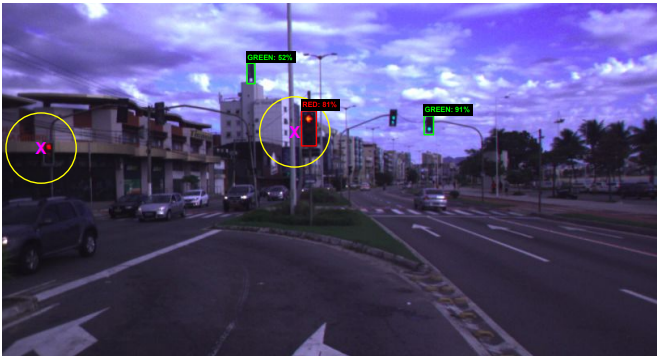
\includegraphics[width=\columnwidth]{figures/example/fig05.png}
  \caption{Пример работы системы: 3D-координаты релевантных светофоров с лидара проецируются в 2D-координаты кадра и вокруг них строится 1.5-метровая сфера; релевантными светофорами в кадре считаются те, чьи центры попадают в эту сферу и максимально близко лежат к центру реального светофора}
  \label{fig:5}
\end{figure}

\begin{figure}[htbp]
  \centering
  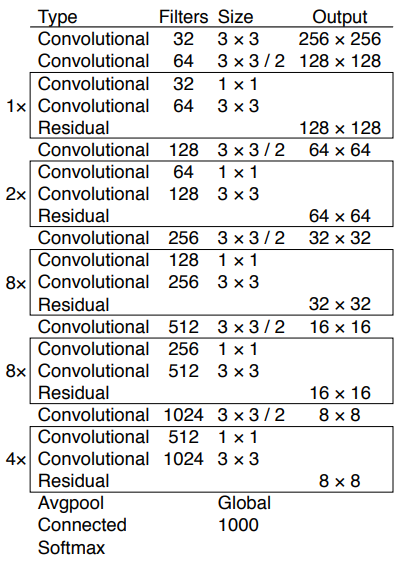
\includegraphics[width=\columnwidth]{figures/example/fig06.png}
  \caption{Архитектура Darknet-53, которая лежит в основе YOLOv3}
  \label{fig:6}
\end{figure}

\subsection{Сочетание SSD-MobileNet V1 и InceptionV3}

Другой подход заключается в использовании MobileNet-SSD для локализации светофоров (нахождение их ограничивающих прямоугольников) и InceptionV3 для распознавания их состояния (цвета). Исходный код доступен по ссылке [17].

MobileNet [20] – эффективная и более лёгкая архитектура нейронной сети, которая может быть использована для классификации или извлечения признаков. Сочетание MobileNet-SSD фактически означает, что для извлечения признаков используется MobileNet (без последнего полносвязного слоя) вместо VGG, а для локализации объекта – SSD.

\begin{figure}[htbp]
  \centering
  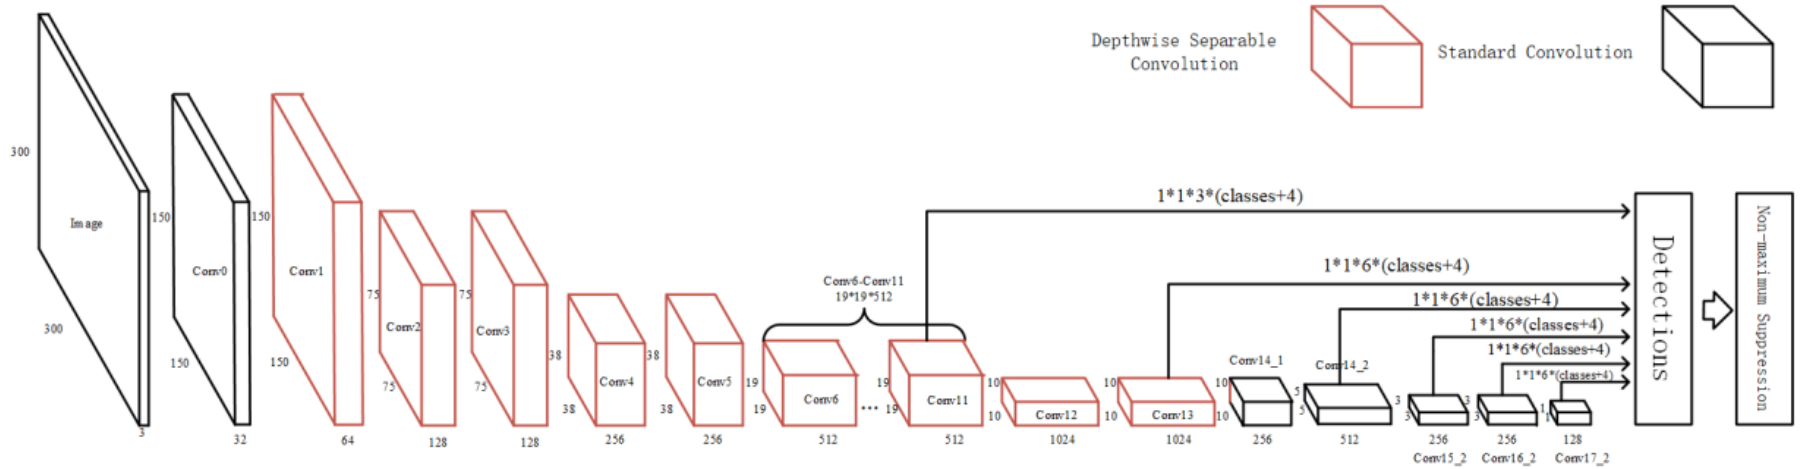
\includegraphics[width=\columnwidth]{figures/example/fig07.png}
  \caption{Архитектура SSD-MobileNetV1}
  \label{fig:7}
\end{figure}

Итоговая архитектура [21] SSD-MobileNetV1 приведена на рисунке 8. Используются веса предобученной на датасете COCO [22] модели.

Для локализованных на кадре светофоров определяется класс их состояния при помощи нейронной сети InceptionV3 [23]. На рисунке 9 приведена архитектура данной сети.

Для классификации используются веса предобученной на наборе данных ImageNet [24] модели, доступные в TensorFlow. Модель дообучается на вырезанных с кадров светофорах набора данных LISA. В качестве функции потерь используется кросс-энтропия в задаче мульклассовой классификации (categorical cross-entropy) – softmax активация в сочетании с кросс-энтропийной функцией потерь. Дообучение длится 10 эпох с размером батча 32. Выходом данной сети является один из 7 классов, которые соответствуют классам в аннотациях набора данных LISA.

\section{Сравнение}

Сравним два описанных подхода. Для сравнения используется часть набора данных LISA – 7473 изображения с 18020 размеченными светофорами. Качество работы двух подходов складывается из качества работы локализующей и классифицирующей частей. Оценка локализации производится при помощи расчёта меры Жаккара (Intersection over Union, IoU) для каждой детекции. Найденные детектором светофоры связываются с существующей разметкой с порогом 10\%. Введём следующие величины:

Разработка конечной системы велась в две стадии:

TP – детектор верно локализовал светофор (найдена соответствующая разметка – прямоугольники разметки и детекции пересекаются более, чем на 10\%, по отношению к их общей площади).

FP – детектор нашёл светофор там, где его нет, то есть не найдено такого прямоугольника в разметке кадра, который пересекался бы с найденным более, чем на 10\%.

FN – детектор не нашёл светофор, хотя он есть и для него есть разметка – пересечение менее, чем 10\%.

Стоит отметить, что TN в данном случае не определена, так как это величина означает то, что детектор не определил светофор, где его действительно нет. По введённым величинам строятся такие функции оценок, как:

– сколько раз детектор нашёл светофор, где он действительно есть, по отношению к общему числу предсказанных светофоров;

– сколько светофоров нашёл детектор из действительно присутствующих в кадрах;

– оценка баланса между точностью (precision) и полнотой (recall).

\begin{figure}[htbp]
  \centering
  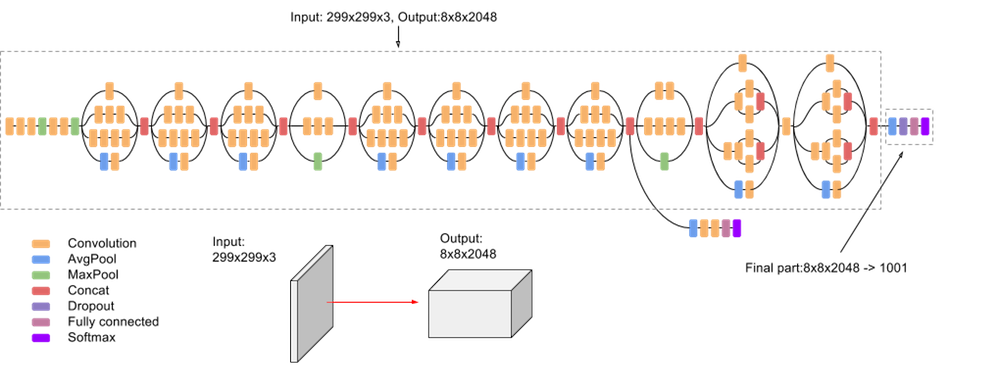
\includegraphics[width=\columnwidth]{figures/example/fig08.png}
  \caption{Архитектура InceptionV3}
  \label{fig:8}
\end{figure}

Также в случае с видеопоследовательностями, можно использовать функции MOT [25] – MOTA (multiple object tracking accuracy), которая оценивает общую точность отслеживания и детекции, и MOTP (multiple object tracking precision) – оценка точности локализации светофоров (схожа с метрикой mAP [16]). Формулы (2) и (3) соответствуют формулам данных функций. При этом значения функции MOTA могут быть отрицательными – область значений .

Здесь IoUi – мера Жаккара i-го объекта на всей тестовой выборке. GT означает суммарное количество аннотаций, а IDS – количество потерь трека светофоров. В нашем случае показатель IDS не важен, так как производится оценка именно локализации, поэтому эта величина не участвует при расчёте показателя MOTA. Таблица 1 отображает количественные оценки для двух подходов.

\begin{table}[htbp]
  \caption{Оценка детектирующей части}
  \label{tab:detector}
  \centering
  \begin{tabular}{lcc}
    \toprule
    & YOLOv3 (детектор) & SSD-MobileNet V1 \\
    \midrule
    TP & 15420 & 4048 \\
    FP & 2095 & 12276 \\
    FN & 2600 & 13972 \\
    Precision & 0.88 & 0.25 \\
    Recall & 0.86 & 0.22 \\
    F1 & 0.87 & 0.24 \\
    MOTA & 0.74 & $-$0.46 \\
    MOTP & 0.59 & 0.44 \\
    \bottomrule
  \end{tabular}
\end{table}

Как видно из таблицы детектор YOLOv3 имеет значительно более высокие показатели, что означает, что он намного больше находит действительных светофоров и намного меньше ошибается, детектируя не относящееся к делу окружение. Примечательно, что значение функции MOTA для YOLOv3 достаточно близко к 1, в то время как оценка для SSD-MobileNet V1 имеет отрицательное значение.

В оценку классифицирующей части включены все объекты, которые входят в множество TP локализующей части. Классифицирующая нейронная сеть InceptionV3 второго подхода на выходе имеет 7 классов, в то время как классификатор YOLOv3 предсказывает всего 2. Связи с этим матрицы ошибок имеют разные размеры. На рисунке 10 отображена матрица ошибок и отчёт о классификации, содержащий precision, recall и F1-меру [26, 27], для нейросети InceptionV3. Здесь номера классов 0–6 означают состояния светофора go, goForward, goLeft, stop, stopLeft, warning, warningLeft соответственно.

\begin{figure}[htbp]
  \centering
  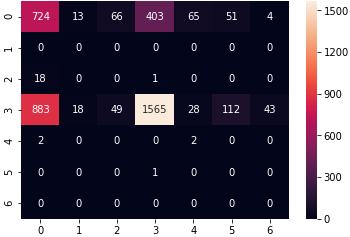
\includegraphics[width=\columnwidth]{figures/example/fig09.png}
  \caption{Матрица ошибок и численная оценка работы InceptionV3}
  \label{fig:9}
\end{figure}

Как можно видеть, классы go и stop хоть и распознаются с не очень высоким значением F1-меры, но остальные классы не распознаются вообще. Такую оценку можно объяснить тем, что для большого количества классов и достаточного качества их распознавания очень важно иметь широкую и сбалансированную обучающую выборку. Такой выборки не было зафиксировано на этапе обучения данной сети.

Классифицирующая часть YOLOv3 на выходе имеет всего 2 класса. Поэтому можно определить некоторую переходную матрицу ошибок (рисунок 11а), которая содержала бы 7 реальных классов и 2 класса предсказываемых. Но больший смысл будет иметь матрица ошибок в обычном смысле (рисунок 11б) – здесь реальные классы go, goForward и goLeft объединены в класс go (метка 0), а классы stop, stopLeft, warning и warningLeft объединены в класс stop с меткой 1.

Численные оценки классификации этой нейросети имеют значения, близкие к 100\% (рисунок 12). Такую сильную с предыдущей нейронной сетью разницу в качестве можно объяснить несколькими обстоятельствами: более долгое обучение на более релевантных наборах данных, меньшее число предсказываемых классов, более сбалансированная и широкая обучающая выборка, большее число тестовых картинок, так как более качественный детектор смог правильно локализовать большее число светофоров, которые затем и классифицировались.

Сравнивая классификаторы YOLOv3 и InceptionV3, можно заметить, что классы go и stop, наиболее широко представленные в датасете LISA, InceptionV3 распознаёт лучше всего. YOLOv3 распознаёт эти классы тоже хорошо (и даже лучше из-за упомянутых обстоятельств), но в случае с YOLOv3 лучше подготовлены данные для обучения. Это ещё раз показывает важность составления репрезентативной, широкой и сбалансированной обучающей выборки.

\begin{figure}[htbp]
  \centering
  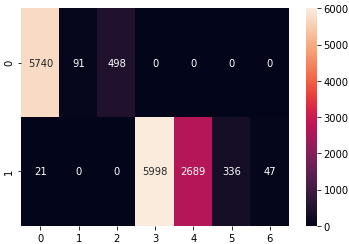
\includegraphics[width=\columnwidth]{figures/example/fig10.png}
  \caption{Переходная 2х7 и обычная матрицы ошибок 2х2 нейросети YOLOv3}
  \label{fig:10}
\end{figure}

\begin{figure}[htbp]
  \centering
  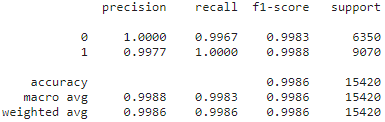
\includegraphics[width=\columnwidth]{figures/example/fig11.png}
  \caption{Численная оценка качества работы классификатор YOLOv3}
  \label{fig:11}
\end{figure}

\section{Заключение}

Были рассмотрены основные наборы данных, на которых обучались и тестировались рассматриваемые нейронные сети. Приведены два подхода к детектированию – локализации и классификации – светофоров: YOLOv3, предложенная и обученная авторами работы [14], в которой решалась задача определения состояния релевантных светофоров, и сочетание предобученных SSD-MobileNet V1 и InceptionV3 [17]. Каждая сеть рассмотрена с точки зрения её архитектуры, процесса обучения, используемых для обучения и тестирования наборов данных.

Приведённые подходы были сравнены на части датасета LISA. Отдельно были оценены качество локализации и классификации светофоров. По полученным данным очевидно, что нейронная сеть YOLOv3, подготовленная авторами работы [14], имеет сильное преимущество перед альтернативным подходом, что объясняется разными обучающими процессами и разным качеством обучающих выборок. Притом сравнивались именно конкретные модели с конкретными весами. Для сравнения архитектур в целом нужны фиксированные наборы и процессы обучения и тестирования.

\begin{thebibliography}{99}

\bibitem{ref1}
“Driverless cars (global market)”, available at: https://www.tadviser.ru/index.php/Статья:Беспилотные\_автомобили\_(мировой\_рынок) (Accessed: December 25, 2022).

\bibitem{ref2}
Jensen M.B., Philipsen M.P., Møgelmose A., Moeslund T.B., Trivedi M.M. “Vision for looking at traffic lights: Issues, survey, and perspectives”, IEEE Transactions on Intelligent Transportation Systems, 2016, no. 17, pp. 1800–181.

\bibitem{ref3}
Verma, M.P. and Singh, V.B.P. (2016) Traffic light recognition system: A computer vision based approach, International Journal For Science Technology And Engineering. Available at: https://ijste.org/Article.php?manuscript=IJSTEV3I3035 (Accessed: December 25, 2022).

\bibitem{ref4}
R. F. Berriel, A. T. Lopes, A. F. de Souza, and T. Oliveira-Santos, “Deep Learning Based Large-Scale Automatic Satellite Crosswalk Classification,” IEEE Geoscience and Remote Sensing Letters, vol. 14, pp. 1513–1517, Sept 2017.

\bibitem{ref5}
R. F. Berriel, F. S. Rossi, A. F. de Souza, and T. Oliveira-Santos, “Automatic Large-Scale Data Acquisition via Crowdsourcing for Crosswalk Classification: A Deep Learning Approach,” Computers \& Graphics, vol. 68, pp. 32–42, Nov 2017.

\bibitem{ref6}
R. Guidolini, L. G. Scart, L. F. R. Jesus, V. B. Cardoso, C. Badue, and T. Oliveira-Santos, “Handling Pedestrians in Crosswalks Using Deep Neural Networks in the IARA Autonomous Car,” in 2018 International Joint Conference on Neural Networks (IJCNN), pp. 1–8, July 2018.

\bibitem{ref7}
J. Redmon, S. Divvala, R. Girshick, and A. Farhadi, “You only look once: Unified, real-time object detection,” in Proceedings of the IEEE conference on computer vision and pattern recognition, pp. 779–788, 2016.

\bibitem{ref8}
S. Ren, K. He, R. Girshick, and J. Sun, “Faster R-CNN: Towards realtime object detection with region proposal networks,” in Advances in neural information processing systems, pp. 91–99, 2015.

\bibitem{ref9}
Jensen M.B., Philipsen M.P., Møgelmose A., Moeslund T.B., Trivedi M.M. “Vision for looking at traffic lights: Issues, survey, and perspectives”, IEEE Transactions on Intelligent Transportation Systems, 2016, no. 17, pp. 1800–1815.

\bibitem{ref10}
Behrendt K., Novak L., Botros R. “A deep learning approach to traffic lights: Detection, tracking, and classification”, 2017 IEEE International Conference on Robotics and Automation (ICRA), 2017, pp. 1370–1377.

\bibitem{ref11}
Yu F., Xian W., Chen Y., Liu F., Liao M., Madhavan V., Darrell T. “Bdd100k: A diverse driving video database with scalable annotation tooling”, arXiv preprint arXiv, 2018, 1805.04687.

\bibitem{ref12}
A. Fregin, J. Muller, U. Krebel and K. Dietmayer, "The DriveU Traffic Light Dataset: Introduction and Comparison with Existing Datasets," 2018 IEEE International Conference on Robotics and Automation (ICRA), 2018, pp. 3376-3383.

\bibitem{ref13}
R. Hamzah, H. Ibrahim, "Literature Survey on Stereo Vision Disparity Map Algorithms", Journal of Sensors, 2016, pp. 1-23.

\bibitem{ref14}
Possatti, Lucas C. et al. “Traffic Light Recognition Using Deep Learning and Prior Maps for Autonomous Cars”, 2019 International Joint Conference on Neural Networks (IJCNN), 2019, pp. 1-8.

\bibitem{ref15}
J. Redmon, A. Farhadi. “YOLOv3: An Incremental Improvement”, ArXiv abs/1804.02767, 2018, pp. 1-6.

\bibitem{ref16}
M. Everingham, L. Van Gool, Williams, C.K.I. et al. “The PASCAL Visual Object Classes (VOC) Challenge”, International Journal of Computer Vision, 2010, vol. 88, pp. 303–338.

\bibitem{ref17}
SSD-MobileNet V1 detection and InceptionV3 classification source code, available at: https://www.kaggle.com/code/chandanakuntala/detection-classification-of-traffic-lights/notebook\#CLASSIFICATION (Accessed: December 25, 2022).

\bibitem{ref18}
W. Liu, D. Anguelov, D. Erhan et al. “SSD: Single Shot MultiBox Detector”, European Conference on Computer Vision, 2015, pp. 1-17.

\bibitem{ref19}
K. Simonyan, A. Zisserman. “Very Deep Convolutional Networks for Large-Scale Image Recognition”, The 3rd International Conference on Learning Representations (ICLR2015), 2014, pp. 1-14.

\bibitem{ref20}
A. G. Howard et al. “MobileNets: Efficient Convolutional Neural Networks for Mobile Vision Application.,” Howard, Andrew G., et al. "Mobilenets: Efficient convolutional neural networks for mobile vision applications." arXiv preprint arXiv:1704.04861, 2017, pp. 1-9.

\bibitem{ref21}
C. Xu and Y. Mao, “An improved traffic congestion monitoring system based on federated learning”, Information, 2020, vol. 11, no. 7, pp. 1–22.

\bibitem{ref22}
T. Lin, M. Maire, S. J. Belongie, Hays et. al. “Microsoft COCO: Common Objects in Context. European Conference on Computer Vision”, Computer Vision (ECCV2014), 2014, vol. 8693, pp. 740-755.

\bibitem{ref23}
C. Szegedy, V. Vanhoucke, S. Ioffe et. al. “Rethinking the Inception Architecture for Computer Vision”, 2016 IEEE Conference on Computer Vision and Pattern Recognition (CVPR), 2015, pp. 2818-2826.

\bibitem{ref24}
J. Deng, W. Dong, R. Socher, L. -J. Li, Kai Li and Li Fei-Fei, "ImageNet: A large-scale hierarchical image database", 2009 IEEE Conference on Computer Vision and Pattern Recognition, 2009, pp. 248-255.

\bibitem{ref25}
J. Luiten, A. Os̆ep, P. Dendorfer et al. “HOTA: A Higher Order Metric for Evaluating Multi-object Tracking”, International Journal of Computer Vision, 2021, vol. 129, pp. 548–578.

\bibitem{ref26}
Z. C. Lipton, C. P.Elkan, B. Narayanaswamy. “Thresholding Classifiers to Maximize F1 Score”, 2014 arXiv: Machine Learning, pp. 1-16.

\bibitem{ref27}
M. Sokolova, N. Japkowicz, S. Szpakowicz. “Beyond accuracy, F-score and ROC: a family of discriminant measures for performance evaluation”, Proceedings of Australasian joint conferenceon artificial intelligence, 2006, vol. 4304, pp. 1015-1021.

\end{thebibliography}

\end{document}
